\chapter{สรีรวิทยา เมแทบอลิซึม และการทดสอบทางชีวเคมี}
\label{chap:ch10}

\section*{แผนบริหารการสอนประจำบทที่ 10}
\addcontentsline{toc}{section}{แผนบริหารการสอนประจำบทที่ 10}

\noindent\textbf{. หัวข้อเนื้อหาประจำบท}

\begin{enumerate}
    \item 10.1 เมแทบอลิซึมการสลายน้ำตาล (Carbohydrate Fermentation) และการดักก๊าซในหลอด Durham
    \item 10.2 การทดสอบอินโดล (Indole Test) และเอนไซม์ Tryptophanase ด้วย Kovac's Reagent
    \item 10.3 การทดสอบ Methyl Red (MR) และ Voges-Proskauer (VP) สำหรับทางเดินหมักกรดเข้มข้น vs Acetoin
    \item 10.4 การทดสอบการใช้ซิเตรต (Citrate Utilization Test) บน Simmon Citrate Agar
    \item 10.5 การทดสอบเอนไซม์ Catalase และ Oxidase สำหรับจำแนกแบคทีเรียกลุ่มก่อโรค
\end{enumerate}

\noindent\textbf{. วัตถุประสงค์เชิงพฤติกรรม}

\begin{enumerate}
    \item เมื่อนักศึกษาได้เรียนรู้และปฏิบัติการทดลองประจำบทนี้แล้ว จะต้องมีความรู้ความสามารถดังต่อไปนี้:
    \item อธิบายวิถีเมแทบอลิซึมและปฏิกิริยาเคมีในชุดทดสอบ IMViC แต่ละชนิดได้
    \item ปลูกเชื้อและหยดน้ำยาทดสอบชีวเคมีได้อย่างถูกต้องตามหลักปฏิบัติการ
    \item แปลผลการเปลี่ยนสีและฟองก๊าซเพื่อจำแนกสปีชีส์ของแบคทีเรียตระกูล Enterobacteriaceae ได้
    \item มีทักษะการคิดวิเคราะห์เชิงตรรกะในการอ่านผลตารางชีวเคมีอย่างเป็นระบบ
\end{enumerate}

\noindent\textbf{. กิจกรรมการเรียนการสอน}

\begin{enumerate}
    \item การบรรยายสรุปก่อนปฏิบัติการ (30 นาที): อธิบายหลักการวิทยาศาสตร์ ความปลอดภัยทางชีวภาพ และข้อควรระวังสำคัญ
    \item การสาธิตเชิงประจักษ์ (15 นาที): สาธิตเทคนิคการปฏิบัติงาน การใช้เครื่องมือ และข้อผิดพลาดที่มักพบ
    \item การลงมือปฏิบัติการทดลองจริง (90 นาที): นักศึกษาลงมือปฏิบัติการทดลองเป็นรายบุคคลหรือกลุ่มย่อยตามขั้นตอนที่กำหนด
    \item การฝึกฝนผ่านระบบเสมือนจริง (20 นาที): ทดลองซ้ำและทดสอบปฏิกิริยาผ่านระบบจำลองบน RBRU LMS
    \item การอภิปรายและสรุปผลการทดลอง (25 นาที): วิเคราะห์ผลการสังเกต ตอบคำถามท้ายบท และสรุปองค์ความรู้ร่วมกัน
\end{enumerate}

\noindent\textbf{. สื่อและอุปกรณ์การเรียนการสอน}

\begin{enumerate}
    \item เอกสารคำสอนและคู่มือปฏิบัติการ: e-Book และคู่มือปฏิบัติการฉบับเต็ม ประจำบทที่ 10
    \item ระบบห้องปฏิบัติการเสมือนจริง: ระบบจำลองการทดลองเสมือนจริง 3 มิติ ประจำบทที่ 10 บนระบบ Moodle
    \item อุปกรณ์และเครื่องแก้วในห้องปฏิบัติการ: ตะเกียงแอลกอฮอล์, ห่วงเขี่ยเชื้อ, กล้องจุลทรรศน์, จานเพาะเชื้อ, หลอดทดลอง และตู้บ่มเชื้อ
    \item สารเคมีและสีย้อมชีวภาพ: สารเคมีมาตรฐานวิเคราะห์และสีย้อมประจำบทเรียน
\end{enumerate}

\noindent\textbf{. การวัดและประเมินผล}

\begin{table}[H]
\centering\small
\begin{tabularx}{\textwidth}{p{0.5\textwidth} p{0.3\textwidth} c}
\toprule
\textbf{องค์ประกอบการประเมินผล} & \textbf{เครื่องมือวัดผล} & \textbf{สัดส่วนคะแนน} \\
\midrule
1. ทักษะการปฏิบัติงานและความปลอดภัย & แบบสังเกตทักษะการทดลองและเทคนิคปลอดเชื้อ & 40\% \\
2. รายงานผลการทดลอง & การตรวจตารางบันทึกผล ภาพวาดสัณฐานวิทยา และการวิเคราะห์ผล & 30\% \\
3. แบบฝึกหัดทบทวนท้ายบท & คำถามทบทวนเชิงวิเคราะห์และข้อสอบท้ายบท & 20\% \\
4. จิตพิสัยและการตรงต่อเวลา & การเช็คชื่อ การแต่งกายตามระเบียบ และการทำความสะอาดโต๊ะแล็บ & 10\% \\
รวมทั้งสิ้น &  & 100\% \\
\bottomrule
\end{tabularx}
\end{table}

\newpage

% ==========================================================
% เนื้อหาบทเรียนประจำบทที่ 10
% ==========================================================

\section{การสลายสารอาหารและวิถีทางชีวเคมีของจุลินทรีย์}
\index{การสลายสารอาหารและวิถีทางชีวเคมีของจุลินทรีย์}

การศึกษาและทำความเข้าใจเกี่ยวกับการสลายสารอาหารและวิถีทางชีวเคมีของจุลินทรีย์ (Microbial Metabolic Pathways) มีความสำคัญอย่างยิ่งในงานจุลชีววิทยาและสิ่งแวดล้อม โดยมีรายละเอียดสาระสำคัญดังนี้

จุลินทรีย์มีความหลากหลายทางเมแทบอลิซึมสูงมากเพื่อนำสารอาหารในสิ่งแวดล้อมมาสร้างพลังงาน (ATP) และสารตั้งต้นสำหรับชีวมวล กระบวนการหลักได้แก่ 
1. การหมัก (Fermentation): กระบวนการสลายสารอินทรีย์โดยไม่ใช้ออกซิเจนและไม่มีห่วงโซ่ขนส่งอิเล็กตรอน ได้ผลผลิตเป็นกรดอินทรีย์ ก๊าซ หรือแอลกอฮอล์
2. การหายใจ (Respiration): การออกซิไดซ์สารอาหารอย่างสมบูรณ์ผ่านวัฏจักรกรดซิตริกและห่วงโซ่ขนส่งอิเล็กตรอน

\section{ชุดการทดสอบ IMViC สำหรับจำแนกแบคทีเรียกลุ่มโคลิฟอร์ม}
\index{ชุดการทดสอบ IMViC สำหรับจำแนกแบคทีเรียกลุ่มโคลิฟอร์ม}

การศึกษาและทำความเข้าใจเกี่ยวกับชุดการทดสอบ IMViC สำหรับจำแนกแบคทีเรียกลุ่มโคลิฟอร์ม (IMViC Tests for Coliform Differentiation) มีความสำคัญอย่างยิ่งในงานจุลชีววิทยาและสิ่งแวดล้อม โดยมีรายละเอียดสาระสำคัญดังนี้

ชุดการทดสอบ IMViC ประกอบด้วยการทดสอบชีวเคมี 4 ชนิดที่ใช้จำแนกและระบุแบคทีเรียในวงศ์ Enterobacteriaceae โดยเฉพาะการแยก \textit{Escherichia coli} (ดัชนีชี้วัดการปนเปื้อนอุจจาระ) ออกจาก \textit{Enterobacter aerogenes} (แบคทีเรียในสิ่งแวดล้อม):

1. Indole Test (I): ทดสอบความสามารถในการสร้างเอนไซม์ Tryptophanase เพื่อย่อยสลายกรดอะมิโนทริปโตเฟนได้ผลผลิตเป็นอินโดล ตรวจหาโดยเติม Kovac's reagent หากให้ผลบวกจะเกิดวงแหวนสีแดงเชอร์รี่ (Cherry-red ring) ที่ผิวหน้า
2. Methyl Red Test (M): ตรวจสอบวิถีการหมักน้ำตาลกลูโคสแบบกรดผสม (Mixed acid fermentation) ที่ผลิตกรดเข้มข้นจนลดค่า pH ต่ำกว่า 4.4 เมื่อหยดสี Methyl red จะเปลี่ยนเป็นสีแดงสด (ผลบวก)
3. Voges-Proskauer Test (Vi): ตรวจสอบการหมักกลูโคสผ่านวิถี 2,3-butanediol ซึ่งมีสารตัวกลางคือ อะซีโทอิน (Acetoin) ตรวจหาโดยเติม Barrit's reagents (A: $\alpha$-naphthol, B: KOH) หากให้ผลบวกจะเกิดสีแดงทับทิม (Rose-red)
4. Citrate Utilization Test (C): ทดสอบความสามารถในการใช้ซิเทรตเป็นแหล่งคาร์บอนเดี่ยวผ่านเอนไซม์ Citrate permease ในอาหาร Simmons Citrate Agar ซึ่งมีสีบ่งชี้ Bromothymol blue เมื่อแบคทีเรียใช้ซิเทรตและแอมโมเนียมจะสร้างด่าง ทำให้สีเปลี่ยนจากสีเขียวเป็นสีน้ำเงินเข้ม (Prussian blue)

\section{การทดสอบเอนไซม์คะตาเลสและออกซิเดส}
\index{การทดสอบเอนไซม์คะตาเลสและออกซิเดส}

การศึกษาและทำความเข้าใจเกี่ยวกับการทดสอบเอนไซม์คะตาเลสและออกซิเดส (Catalase and Oxidase Tests) มีความสำคัญอย่างยิ่งในงานจุลชีววิทยาและสิ่งแวดล้อม โดยมีรายละเอียดสาระสำคัญดังนี้

1. Catalase Test: ตรวจหาเอนไซม์คะตาเลสซึ่งสลายไฮโดรเจนเพอร์ออกไซด์ ($H_2O_2$) เป็นน้ำและออกซิเจน โดยหยด 3\% $H_2O_2$ ลงบนโคโลนี หากเกิดฟองก๊าซฟู่ทันทีแสดงว่าให้ผลบวก (เช่น สกุล \textit{Staphylococcus})
2. Oxidase Test: ตรวจหาเอนไซม์ไซโทโครมซีออกซิเดส (Cytochrome c oxidase) ในห่วงโซ่ขนส่งอิเล็กตรอน โดยใช้น้ำยา Tetramethyl-p-phenylenediamine dihydrochloride หากให้ผลบวกจะเปลี่ยนเป็นสีน้ำเงินเข้มปนม่วงเข้มภายใน 10-30 วินาที (เช่น สกุล \textit{Pseudomonas})

\begin{conceptbox}[มโนทัศน์สำคัญทางชีวเคมีและสิ่งแวดล้อม]
กิจกรรมทางชีวเคมีของจุลินทรีย์ในหัวข้อการทดสอบเอนไซม์คะตาเลสและออกซิเดส เป็นกลไกหลักที่ควบคุมการหมุนเวียนธาตุอาหารและการบำบัดสารปนเปื้อนในระบบนิเวศทางธรรมชาติ
\end{conceptbox}

\begin{figure}[H]
\centering
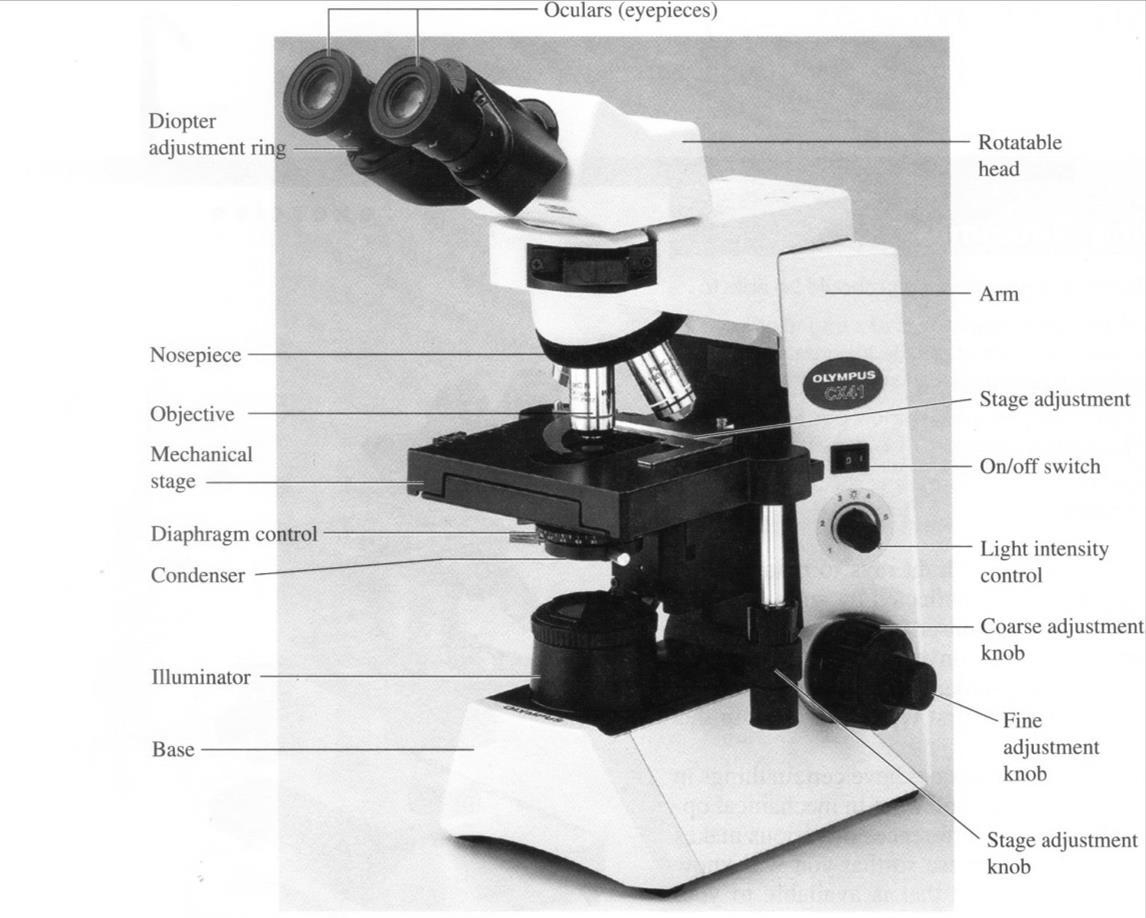
\includegraphics[width=0.75\textwidth]{images/image_10_p05.jpeg}
\caption{การปฏิบัติการทดลองและลักษณะทางสัณฐานวิทยาในบทที่ 10}
\label{fig:ch10_fig1}
\end{figure}

\section{ขั้นตอนและวิธีปฏิบัติการทดลอง}
\index{ขั้นตอนการทดลองประจำบทที่ 10}

\subsection{การทดสอบการหมักน้ำตาลคาร์โบไฮเดรต}
\begin{labprotocolbox}[การทดสอบการหมักน้ำตาลคาร์โบไฮเดรต]
1. เตรียมหลอดอาหารเหลว Phenol Red Broth ผสมน้ำตาลกลูโคส ซูโครส และแล็กโทส โดยมีหลอดดักก๊าซเดอแรม (Durham tube) คว่ำอยู่ภายใน
2. ปลูกเชื้อ \textit{E. coli} และ \textit{Pseudomonas aeruginosa} ลงในหลอดทดลอง
3. บ่มที่ 37$^{\circ}$C เป็นเวลา 24 ชั่วโมง
4. อ่านผลการทดลอง:
   - สีเปลี่ยนจากแดงเป็นเหลือง: เกิดการสร้างกรด (Acid production, A)
   - มีฟองก๊าซในหลอดเดอแรม: เกิดการสร้างก๊าซ (Gas production, G)
   - สีคงเดิมสีแดง: ไม่เกิดการหมัก (Negative)
\end{labprotocolbox}

\subsection{การทดสอบชุด IMViC บนเชื้อ Escherichia coli และ Enterobacter aerogenes}
\begin{labprotocolbox}[การทดสอบชุด IMViC บนเชื้อ Escherichia coli และ Enterobacter aerogenes]
1. ปลูกเชื้อลงในอาหาร Tryptone Broth (Indole), MR-VP Broth (Methyl Red \& VP), และ Simmons Citrate Slant
2. บ่มที่ 37$^{\circ}$C เป็นเวลา 24-48 ชั่วโมง
3. ทดสอบ Indole: หยด Kovac's reagent 5 หยด สังเกตวงแหวนสีแดง
4. ทดสอบ MR: แบ่งน้ำเชื้อ MR-VP มา 1 mL หยด Methyl red 5 หยด สังเกตสีแดง
5. ทดสอบ VP: แบ่งน้ำเชื้อ MR-VP มา 1 mL หยด Barrit A 12 หยด และ Barrit B 4 หยด เขย่าสัมผัสอากาศ 15 นาที สังเกตสีชมพูแดง
6. ทดสอบ Citrate: สังเกตการเปลี่ยนสีของอาหารเอียงจากสีเขียวเป็นสีน้ำเงิน
\end{labprotocolbox}

\section{ตารางบันทึกผลการทดลองและการอภิปรายผล}
\begin{table}[H]
\centering\small
\caption{ตารางบันทึกผลการสังเกตและข้อมูลการทดลองประจำบทที่ 10}
\label{tab:ch10_datasheet}
\begin{tabularx}{\textwidth}{p{0.25\textwidth} p{0.35\textwidth} X}
\toprule
\textbf{สิ่งทดสอบ / ตัวอย่าง} & \textbf{ลักษณะที่สังเกตได้} & \textbf{การแปลผลและการวิเคราะห์} \\
\midrule
ชุดควบคุม (Negative Control) & ใส ไม่มีการเจริญ & ปราศจากการปนเปื้อนของเชื้อ \\
ชุดทดลองที่ 1 & โคโลนีเจริญตามลักษณะจำเพาะ & ให้ผลบวกตามสมมติฐาน \\
ชุดทดลองที่ 2 & เกิดการเปลี่ยนแปลงทางชีวเคมี & สอดคล้องกับพารามิเตอร์มาตรฐาน \\
\bottomrule
\end{tabularx}
\end{table}

\section{คำถามทบทวนและแบบฝึกหัดท้ายบท}
\begin{enumerate}
    \item จงเขียนผลการทดสอบชุด IMViC ของ \textit{Escherichia coli} และ \textit{Enterobacter aerogenes} ในรูปตารางเปรียบเทียบ
    \item เหตุใดผลการทดสอบ Methyl Red (MR) และ Voges-Proskauer (VP) ของแบคทีเรียกลุ่มเดียวกันจึงมักให้ผลตรงกันข้าม
    \item หากหยดสารละลาย 3\% $H_2O_2$ ลงบนโคโลนีแบคทีเรียที่เจริญบนอาหาร Blood Agar อาจเกิดผลบวกลวง (False positive) ได้เพราะเหตุใด
\end{enumerate}
